
\section{Exercícios}
\begin{frame}
	\frametitle{Exercícios} 
	
	\setcounter{exercicios}{12}
	\begin{exercicio}
		Dada as frações $$\frac{966666555557}{966666555558} \; \text{ e
	} \; \frac{966666555558}{966666555559},$$ qual é a maior?
	\end{exercicio} 
	
	\Ex{Nove cópias de certas notas custam menos de R\$ 10,00 e dez
	cópias das mesmas notas (custando o mesmo preço cada uma) custam
	mais de R\$ 11,00. Quanto custa uma cópia das notas? }
	
\end{frame}
	
	
%------------------------------------------------------------------------------------------------------------
\begin{frame}
\frametitle{Exercícios} 
	
	\Ex{ Ache os valores de $x$ para os quais cada uma das seguintes
	inequações é válida:
	\begin{enumerate}[a)]
		\item $ x^2-9  \geq 0$;
		\item $\dfrac x {x^2+9}>0$;
		\item $\dfrac{x-3}{x+1}>0$;
		\item $\dfrac{x^2-1}{x^2-3}>0$;
		\item $\dfrac{x^2+x-6}{x^2+6x+5} \leq 0$;
		\item $\dfrac{-x^2-x+6}{x^2-5x+4} \leq 0$.
	\end{enumerate}
	}
	
	
	
	
	\Ex{
		Para quais valores de $a \pertence \R$ a expressão quadrática $ax^2 - ax +8$ é sempre diferente de zero?
	}

\end{frame}
	
	
%------------------------------------------------------------------------------------------------------------

\begin{frame}
	\frametitle{Exercícios} 
	
	\Ex{ Sejam  $a$, $b$, $c$, $d \in \R\positivos$ tais que $\frac a b < \frac c d$.
	Mostre que $$\frac a b < \frac {a+c} {b+d} < \frac c d.$$ }


	
	\Ex{
		Mostre que se $r$ e $s$ são números racionais positivos satisfazendo $r<s$, então existe um outro número racional $q$ tal que $r<q<s$.
	}
	
	\Ex{ Com algarismos $x$, $y$ e $z$ não todos nulos formam-se os
	números de dois algarismos $xy$ e $yx$, cuja soma é o número de três
	algarismos $zxz$. Quanto valem $x$, $y$ e $z$?}
	
	\Ex{ Quantos são os números inteiros de 2 algarismos que são iguais
	ao dobro do produto de seus algarismos?}
	
	
\end{frame}
	
	
%------------------------------------------------------------------------------------------------------------

\begin{frame}
	\frametitle{Exercícios} 
	
	\Ex{ Determine o conjunto solução de cada uma das equações ou
	inequações modulares abaixo:
	\begin{enumerate}[a)]
		\item $\modu {3x - 5}= 7$;
		\item $\modu {-x +8} = -1$;
		\item $\left| x^2-9 \right| = 7$;
		\item $\modu{x^2 - 1} = 3$;
		\item $\modu{x +1} + \modu { -3x +2} = 6$;
		\item $\modu{x-1} \cdot \modu{x+2} = 3$;
		\item $\left| 2x - 5 \right| -3 \leq -2$;
		\item $\modu{x^2 - 1} \menorigual 3$;
		\item $\modu{x-1}+ \modu{x+1}>2$;
		\item $\modu{x+1}- \modu{x-1}<-2$.
	\end{enumerate}
	}


	
	\Ex{ Prove que $\modu{x\cdot y } = \modu x \cdot \modu y$ para todo
	$x, y \in \R$. }
	
	
	
	\Ex{Seja $x \in \R$. Mostre que:
	\begin{enumerate}[a)]
		\item $\modu{x-5}<0,1 \implica \modu{2x - 10}< 0,2;$
		\item $\modu{x+3}<0,1 \implica \modu{-\frac 3 2 x + 3 - 7,5}<0,15;$
		\item $\modu{x-2}< \sqrt{5} - 2 \implica \modu{x^2 - 4}< 1;$
		\item $\modu{x-3} < \sqrt{46} - 5 \implica \modu{x^2+4x-21} < 21.$
	\end{enumerate}
	}
\end{frame}
	
	
%------------------------------------------------------------------------------------------------------------

\begin{frame}
	\frametitle{Exercícios} 	
		
	\Ex{
		Quatro cidades rurais, \emph{Abaeté}, \emph{Bertioga}, \emph{Caicó} e \emph{Diamantina}, estão situadas geograficamente como a imagem abaixo.
		\begin{figure}[H]
			\centering
			\label{fig:exercicio-cidades}
			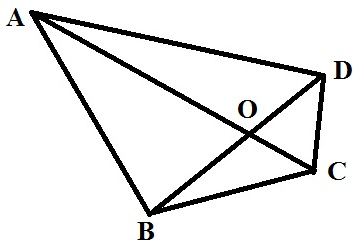
\includegraphics[scale=0.5]{figures/exercicio-cidades.jpg}
			%\caption{Disposição das cidades.}
		\end{figure}
		A empresa \emph{Ozymandias} deseja construir uma central de distribuição de energia para as quatro cidades de modo que a soma total das distâncias da central a cada uma das quatro cidades seja a mínima possível. Mostre que a central deve ser construída no ponto $O$, que é o ponto em comum dos segmentos $AC$ e $BD$.
	}
	
\end{frame}
	
	
%------------------------------------------------------------------------------------------------------------

\begin{frame}
	\frametitle{Exercícios} 
	\Ex{
		Três círculos que não se intersectam tem seus centros colineares (sobre uma mesma reta). Um quarto círculo os tangencia, conforme a imagem abaixo. Mostre que o raio do quarto círculo é maior que pelo menos um dos outros raios.
		\begin{figure}[H]
			\centering
			\label{fig:exercicio-4circulos}
		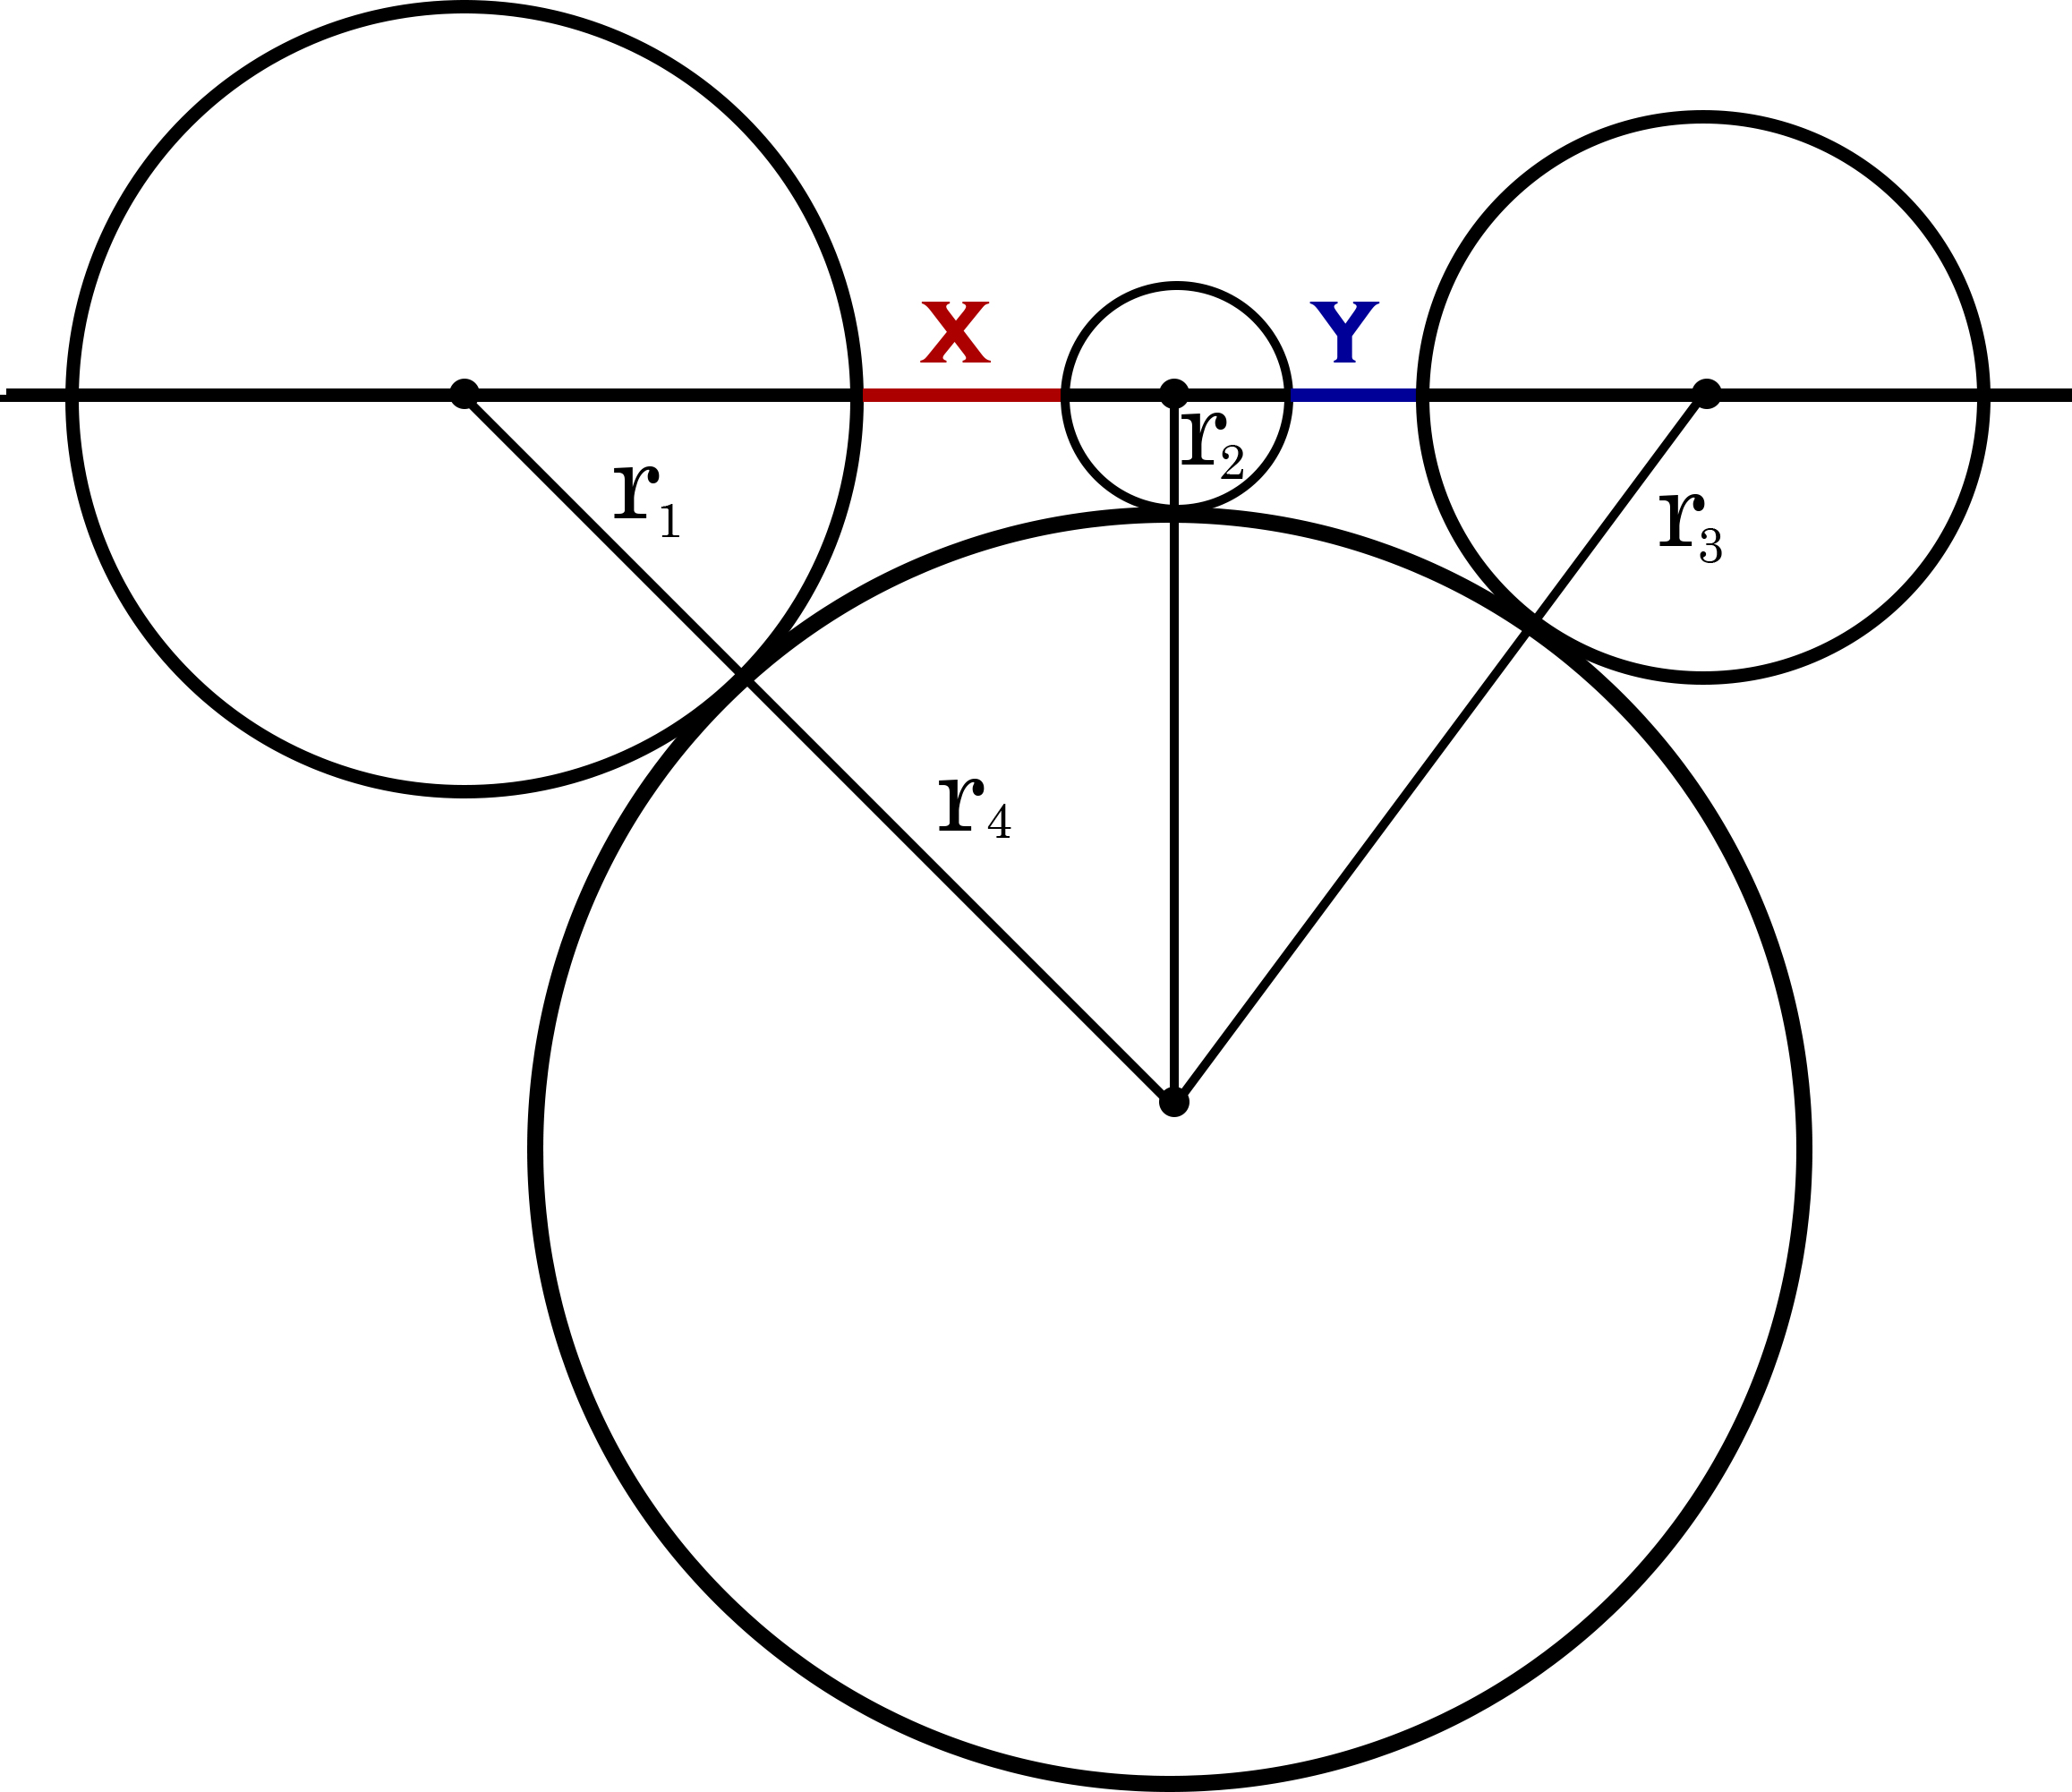
\includegraphics[width=0.6\textwidth]{figures/exercicio-4circulos.jpg}
			\caption{Disposição dos quatro círculos.}
		\end{figure}
	}

	
\end{frame}
	
	
%------------------------------------------------------------------------------------------------------------

\begin{frame}
	\frametitle{Exercícios} 
	
	\Ex{Provar que em todo triângulo a soma dos comprimentos das
	medianas é menor que o perímetro do triângulo e maior que o
	semiperímetro (metade do perímetro) dele. }
	
	\Ex{
		Suponha que $0 < a < b$. Prove que 
		$$a < \sqrt{a \cdot b} < b.$$
	}

	\Ex{
		Sejam $a, b, c \in \R_+^\ast$. Mostre que
        $$\left( ab +bc + ca \right) \geq a\sqrt{bc} + b\sqrt{ac} + c \sqrt{ab}.$$
	}
	
	\Ex{
		Use algum dos resultados da seção de Desigualdades Clássicas e mostre que $4x^3 - 4x^2 + x \geq 0$, para todo $x \geq 0$.
	}
	
	
	\Ex{ Prove que $a^4 +b^4 +c^4 \geq abc \paren{a+b+c}$. }
	
	\Ex{ Sejam $a, b, c \in \R_+$. Prove que $$\paren {a+b} \paren {a+c}
	\paren {b+c} \geq 8abc.$$ }

\end{frame}
	
	
%------------------------------------------------------------------------------------------------------------

\begin{frame}
	\frametitle{Exercícios} 

	\Ex{ Considere $a, b, c \in \R^\ast_+$. Faça o que se pede.
            \begin{enumerate}[a)]
                \item  Use uma das desigualdades das médias para provar que $$a^2b^2c^2 \leq \left( \dfrac {ab+bc+ac} 3  \right)^3;$$
                \item  Considere um paralelepípedo  de lados $a$, $b$ e $c$. Sendo $V$ o volume e $A_L$ a área lateral (área de todas as faces somadas) do paralelepípedo, use o resultado do item anterior (não precisa ter resolvido) para provar que
                $$V \leq \sqrt{\left( \dfrac {A_L} 6  \right)^3} ;$$
                \item  Conclua, a partir dos resultados anteriores, que entre todos os paralelepípedos de área lateral fixada, o de maior volume é o cubo.
            \end{enumerate} }
	
	\end{frame}


	%------------------------------------------------------------------------------------------------------------

\begin{frame}
	\frametitle{Exercícios} 

	\Ex{ Considere $a, b, c, p \in \R^\ast_+$. Faça o que se pede.
            \begin{enumerate}[a)]
                \item  Use uma das desigualdades das médias para provar que, se $\frac p 2 - a, \frac p 2 - b, \frac p 2 - c \in \R^\ast_+$, então $$\left( \dfrac p 2 - a \right)\left( \dfrac p 2 - b \right)\left( \dfrac p 2 - c \right) \leq \left( \frac {\frac p 2 - a + \frac p 2 - b + \frac p 2 - c} 3  \right)^3;$$
                \item  Considere um triângulo de lados $a$, $b$ e $c$, área $A$ e perímetro $p$. A Fórmula de Herón diz que
                $$A = \sqrt{\dfrac p 2 \left( \dfrac p 2 - a \right)\left( \dfrac p 2 - b \right)\left( \dfrac p 2 - c \right)}.$$
                Use o resultado do item anterior para provar que
                $$A \leq \sqrt{\dfrac p 2 \left( \frac {\frac p 2 - a + \frac p 2 - b + \frac p 2 - c} 3  \right)^3} = \dfrac{p^2}{12 \sqrt{3}};$$
                \item  Conclua, a partir dos resultados anteriores, que entre todos os triângulos de perímetro $p$ fixado, o de maior área é o triângulo equilátero.
            \end{enumerate} }
	
	\end{frame}
	
	
	%------------------------------------------------------------------------------------------------------------
	
	\begin{frame}
		\frametitle{Exercícios} 
	
	\Ex{
		Sejam $a_1, a_2, \dots , a_n \pertence \R\positivos$ tais que $a_1 \cdot a_2 \dots a_n =1$. Mostre que
		$$\paren{1+a_1}\cdot\paren{1+a_2}\dots \paren{1+a_n} \geq 2^n.$$
	}
	
	\Ex{ Sejam $a, b, c, d \in \R_+^*$. Prove que $$\paren {a+b+c+d}
	\paren {\frac 1 a + \frac 1 b + \frac 1 c + \frac 1 d} \geq 16.$$ }

\end{frame}
	
	
%------------------------------------------------------------------------------------------------------------

\begin{frame}
	\frametitle{Exercícios} 

	\Ex{
		Considere $n \in \N^\ast$. Faça o que se pede.
		\begin{enumerate}[a)]
			\item  Use as desigualdades das médias para provar que $$1 + \dfrac 1 2 + \dfrac 1 3 + \dots +\dfrac 1 n \geq \dfrac{n^2}{1+2+3+\dots +n};$$
			\item  O somatório dos $n$ primeiros números naturais não nulos é igual a $\dfrac {n(n+1)} 2$. 
			Use o resultado do item anterior (não precisa ter resolvido) para provar que
				$$1 + \dfrac 1 2 + \dfrac 1 3 + \dots +\dfrac 1 n \geq \dfrac{2n}{n+1}.$$
		\end{enumerate}
	}
	
	\Ex{A soma de três números positivos é 6. Prove que a soma de seus
	quadrados não é menor que 12. }
	\end{frame}
	
	%------------------------------------------------------------------------------------------------------------
	
	